
This chapter is the centre part of the thesis. It explains in detail how the method works. It consists of two main sections, the first of which explores in detail what a developer should do while writing the program to minimise the work when debugging. This step is crucial as it is much harder to recreate problems locally as opposed to regular Java applications. The second part focuses on the debugging itself once a developer is informed of an error and has to figure out what is causing it.

\section{Better Developing}
Flink applications are run remotely and without an active user providing input as it is typical for a regular application. Not having a user makes it much harder to recreate the problem as we only have the log files and the stack trace as information. As such it is crucial to have all the information at hand when the program fails, or we notice discrepancies in the resulting data. The only way to make sure that the information is accessible once a problem is reported is to think about what data is necessary for the debugging developer while writing the program. Another issue is that some problems are unique to a distributed environment and won't happen when running on a local host. This section will explain what can be done while writing the program to make the debugging progress much easier.

\subsection{Building Tasks}
The Flink Framework promises a few features that try to set it apart from standard Java applications. These are referenced in \ref{flinkFramework}. The one that sets these applications apart from standard java once while writing the application is the distribution. Applications should be built in a modular way to take full advantage of these features and also make the program easily debuggable.
The development of these tasks should be done using a very similar set of rules as the Unix philosophy states. In fact, Flink modules are not too different to Unix command line tools, they both provide a service while taking an input/output in a predefined way. For the Unix command line, this is the standard output, for Flink programs, these are input and output streams.

\subsubsection{Unix Philosophy}
The Unix philosophy is defined by Doug McIlroy, the inventor of the Unix pipe as follows: \cite{bell1978}
\begin{enumerate}
  \item Make each program do one thing well. To do a new job, build afresh rather than complicate old programs by adding new features.
  \item Expect the output of every program to become the input to another, as yet unknown, program. Don't clutter output with extraneous information. Avoid stringently columnar or binary input formats. Don't insist on interactive input.
  \item Design and build software, even operating systems, to be tried early, ideally within weeks. Don't hesitate to throw away the clumsy parts and rebuild them.
  \item Use tools in preference to unskilled help to lighten a programming task, even if you have to detour to build the tools and expect to throw some of them out after you've finished using them.
\end{enumerate}

Most of the points mentioned here are of some relevance for Flink programming as well. Each task should do one job and do it well. The next paragraph will look into why that is. The second point is necessary by default in Flink, each task has to use the provided streams to work. The third point is equally important if not more important in Flink applications as it is in Unix programs. Always test each Task individually to make sure it works as designed and has no flaws on its own, only then can the whole application work without any problems.

Dividing the program into various modules has a lot of advantages:
\begin{enumerate}
  \item Easier to Develop - It is much simpler to develop a smaller application as it is much harder to lose track of what each piece of code should do. This reduced complexity in return reduces the likelihood of mistakes. Once the program is completed, it results in a more stable program that can be debugged easier.
  \item Better Distribution -  As every Flink task can run on a different computer the smaller the tasks are, the better the Flink Job Manager can distribute the load evenly between the available resources.
  \item Checkpoints are easy to find - Checkpoints are a core piece of Flink technology. It allows the framework not only to jump back and repeat a failed run without having to restart the whole application but also provides information about which state the application is currently in. This is extremely helpful as a lot of Flink applications only end when the program is cancelled by the user.
\end{enumerate}

The modulation of the program not only helps to achieve the advantages of the framework but also supports with debugging later as a lot of the information needed are gathered at the checkpoints.

\subsubsection{Where to split the program}
It should now be understandable that the programs should be divided into multiple tasks, the next question now is how to break the program to get a simple program where there are enough tasks but not too many as too many would lead to the opposite effect we want to achieve.

\paragraph{Why are too many tasks bad?} When there are too many tasks, it gets even more complicated than when everything would be in its task as basically every line of code would be in a different place. Additionally, it wouldn't increase the performance as each task has some initialisation work that would diminish the performance gain achieved by distributing it perfectly.

It makes sense to use the Unix philosophy of having one task do one thing. In most cases there are some obvious choices as in most Flink programs data is modified or analysed each task could be one transformation of the data. It should also be stated that when ever possible the pre-existing transformation functions of the Flink framework should be used. Only in rare situations is it necessary to implement your own data transformation classes. The predefined classes have the advantage of being extensively tested in different conditions thus the risk of data going missing is extremely low.

\subsection{Metrics}
Now that the architecture of the program is done the next question is what metrics to use in which positions to achieve the optimal security.

Once the program architecture is finished, it makes sense to think about what kind of metrics can be used where. Metrics are used to monitor the program without having to debug it and are crucial in notifying the developer if something looks wrong. The first step is figuring out where to use metrics. A good start is to look at the application in the worst possible way; what is the most likely area that an error will occur, after that it makes sense to surround the area with metrics that will catch and log the gathered data. Another great location for metrics is at positions where the through coming data is simple, and metrics can easily be implemented. This should be the case in between tasks. As optimally each task only does one thing it should be easy to check whether the starting and ending assertions are valid.

\subsection{Logging}
Logging in Flink is straightforward and can is used the same as in every other java program that uses log4j. As Flink already provides the necessary libraries to use log4j all a developer has to do is to write the logging config file. Although the logging process itself is the same as every other Java application, it should not be forgotten to use the different log levels that log4j provides. There is a lot of logging happening out of the box just by the Flink process itself. The six logging levels, from highest to lowest are:
\begin{enumerate}
  \item FATAL - the highest logging level, should only be used when the application cannot continue to work because of an unexpected error.
  \item ERROR - whenever an unexpected exception is thrown it should be logged.
  \item WARN - warnings that could lead to errors later on. These are difficult to think of beforehand but if used correctly are very valuable for the debugging developer.
  \item INFO - relevant information like successful database connections and other milestones in the application to let the reader of a log file understand at which point in an application the program currently is.
  \item DEBUG - should be used to record relevant information along the way that could be useful to a programmer when debugging. This could, for example, contain values of variables like database connection strings.
  \item TRACE - is used to let a developer searching for a bug understand the path the application took. Should be logged into a unique log file as it would flood every other one.
\end{enumerate}

\section{The Debugging Process}

There are multiple reasons how an error might be discovered, the most common one being an exception in a log file. Another option is that the end user of the results finds that some of the results are incorrect. Both of these cases require slightly different handling. An excellent way to start the debug process is by using a modified version of the Traffic approach introduced in \ref{aodZeller}.

\subsection{Track the Problem in the database}
Tracking a problem is essential in every development cycle no matter in which language or with what framework and Flink is no exception. It is crucial for every developer to track the status of problems in Flink applications as it helps to minimise work. Along the already mentioned advantages in chapter \ref{aodZellerTrack}, like having an easily accessible database of open problems and knowing which problems are more important than others, tracking the problems of Flink applications offers some other advantages as well.

\begin{enumerate}
  \item Having access to relevant log files.
  \item Knowing how past problems were solved.
  \item What relevant metrics were when the error occurred.
  \item Which subtask of what task manager failed which allows seeing if problems only occur on one machine.
\end{enumerate}

To achieve these advantages the tracking database needs additionally to the already mentioned fields in \ref{aodZellerTrack} a few additional columns. As soon as a problem is experienced the current log files should be saved so that it is easy for the developer to find the relevant lines in the log file even if he starts debugging months later. Secondly, for the same reason, all appropriate metrics should be saved as well.

The resulting columns now are:

\begin{enumerate}
  \item Description
  \item State
  \item Resolution
  \item Assigned Developer
  \item Severity
  \item Link to logs
  \item Steps that were taken to resolve the problem
  \item Relevant metrics
  \item Task manager that was used
\end{enumerate}

\subsection{Reproduce the failure}
Reproducing the problem is probably the most challenging part of debugging Flink applications. As there is no user to report the problem the only help the debugging developer has is information provided by the problem report from the last chapter.

There are two possibilities how a problem is discovered, and both require different steps to reproduce the problem. The first and more difficult one is that an error in the resulting data is discovered without an exception being recorded in the log files. This means that the program is doing something different then what the developer expected when writing it. The second option to discover a problem is by having an exception showing up in the log file.

\subsubsection{Faulty resulting data}
This section will use the word count application as an example program to debug. Notice that the exact implementation of it is irrelevant at this point. The application is a black box as only the incoming, and resulting data are known. To always have the same expected result the following sentence will be used as an input each time: "Hello hello flink flink flink one two". The expected result would be:
\begin{lstlisting}
  hello - 2, flink - 3, one - 1, two - 1
\end{lstlisting}

\paragraph{} The following text explains the process that is used in this case alongside a diagram: \ref{debuggingFaultyData}

\begin{figure}[h!]
    \centering
      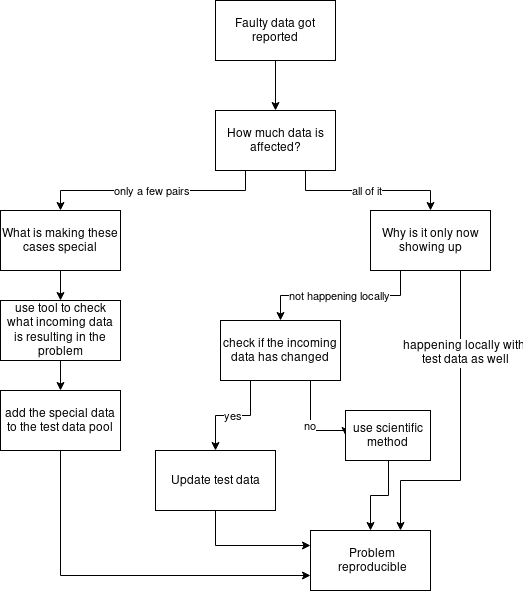
\includegraphics[width=0.9\textwidth]{DebugWithoutException.png}
      \caption{Debbugging faulty data}
      \label{debuggingFaultyData}
\end{figure}

\paragraph{} The first question that has to be answered is
"how much data is affected". Are only a few pieces incorrect or is everything faulty? Imagine the result of the application would be:
\begin{lstlisting}
  hello - 3, flink - 1, one - 1, two - 2
\end{lstlisting}
  Each word has the count of the next word. So this would be considered as the second case "everything is faulty" even though the word "one" has the correct answer. This is important to note as sometimes a fault in a program can still result in a correct result. This first question just differentiates between a few faults and a majority of faults, so the debugging developer has to look at the whole picture and see if the majority of data is corrupt. An example for only a few faults would be:
\begin{lstlisting}
 Hello - 1, hello - 1, flink - 3, one - 1, two - 1
\end{lstlisting}
Here only one additional word was counted ("Hello").
\paragraph{} If the first case is valid (all data is faulty) the next question that should be asked is why the problem is only now showing up. If the problem is observable for almost all the resulting data, surely it should have been noticed while testing the application. In most cases, the problem was either found during testing in which case the problem is already reproducible or was not observable on the local test machine. That means that either the incoming data is different to the local one or that something is being executed differently on the remote network than on the local machine. As Flink is responsible for the distribution and everything is running in a JVM, it is implausible that Flink is to blame. In most cases, the data on the server will differ from the local one. If that can be confirmed the only thing left to do is to update the local test data so that the problem can be reproduced locally.

\paragraph{} The other option was that only some pieces of data were wrong. In that case, the process of reproducing the fault is entirely different. There are two options available. First, figure out what makes the faulty data unique in comparison to the other data. In the word count example, this would be the capital "H" at the beginning of the first "Hello". If this option is successful, the unique case can be added to the test cases, and the reproduction was successful. If on the other hand, the developer can't figure out why the one failing case is different to the others the tool that is written alongside this thesis can be used, it will be explained in detail later on. It can show which incoming data was leading to which result. In the example above it could show that the first "hello" was the result of the original sentence. As there is only one sentence in this example that is not very helpful, but in a more realistic use case, there could be millions of sentences where just a few have capital letters in them. Once the starting sentence is discovered, it can easily be reproduced.

\paragraph{} The last step before moving on to the next section is to make sure that the reproduction works. There is little to no use in finding something in the code that is supposedly the problem only to find out later that the problem is something else.

\paragraph{} The fault should now be reproducible on a local machine as the affecting test data was found. The only fault that remains are problems that only occur on the remote network and are not happening because of differing incoming data. In almost all cases the root of these problems is either incompatible Flink components or network issues. So before starting a more complex search for the problem the developer should check the Flink documentation if all used components, like data sources, the chosen backend etc. are compatible with each other. Furthermore it makes sense to check if all of the running systems can send packages to each other and the database as firewalls and other network related issues could be the issue. If none of these are quickly found it is recommended to use the scientific method described in: \ref{aodZellerIsolateDefect}

\subsubsection{Exception in log file}
The most common way to discover a failure in a program is by discovering an exception. It makes no difference if this exception was found in a log file or directly in the developer's console. The steps that are necessary to reproduce these errors are often easier as well.

\begin{enumerate}
  \item What kind of error was thrown? - The developer should always keep in mind what type of exception was thrown as it is much easier to find the origin of the failure when knowing what to look for.
  \item Where was the failure thrown? - This information is the starting point for the search of how to reproduce the failure. It is included in the stack trace of the exception so it shouldn't be a problem finding it.
  \item Isolate the conditions in the method - Knowing under which conditions the failure occurs is crucial. Without this information, it is almost impossible to reproduce the failure reliably as only a few errors occur under all circumstances. The developer should start by just focusing on the method the exception is thrown in and finding the conditions by looking at the "if statements" that precedent the line in question. Note in which state each variable has to be for the exception to be thrown. This can include the variable that is throwing the exception as well. In most cases, the developer should now already have a pretty good idea as to when the error occurs and if that is the case can skip the next step to save time.
  \item Repeat the same step for the method - Once it is understood in which conditions the failure occurs in the given method, the developer has to find out in which cases the method is being called with the conditions that were deducted in the last step. This can be done by repeating the step above only for the line where the method was called, which is included in the stack trace of the exception as well. This step has to be repeated until the start point of the application has been reached. At this point, the developer should have a good understanding when the exception is thrown and should be able to reproduce it.
\end{enumerate}

\subsubsection{Conclusion}
In most cases, the developer should have no problem reproducing the error easily without going to much in depth into the steps presented in this chapter. Although these steps help to guide a developer that might not even be deeply familiar with the code through the process with ease sometimes problems occur that can not be found using these steps as they are too unique and would not appear for anybody else. If a developer stumbles over such a problem, it is suggested to apply the same method that is explained in \ref{aodZellerIsolateDefect} by creating a hypothesis checking the outcome and repeating the process until the failure can be reproduced.

\subsection{Automate and simplify the test case}
In comparison to typical Java applications where automated testing can be quite tricky as a graphical user interface, and user interaction is involved, automating the test cases for Flink applications is quite easy assuming that the problem is reproducible on a local machine. All that the developer has to do is take the result of the last section and write a test with the specific start parameters. The "Traffic Approach" also suggests simplifying the test case to be as easy to implement as possible so that only the error and nothing else gets checked. This can be useful to make it easier to help spot the problem in the code later on but is not needed for Flink applications. For example, if the word count application were to crash on "-" characters and the input test case would be an entire book page of words it makes it harder later on to find the actual character that is causing the fault but makes it easier to create the test case. As understanding the problem and simplifying the test case is mostly the same it makes sense to leave the test case long and rebuild it once the failure is understood. This way if the same mistake gets built into the code again it is easily spottable as the test case already has a descriptive name, description as well as a ticket number associated with it. Another developer could then easily reproduce the steps that were taken to solve the problem the last time.

\subsection{Find possible infection origins}
This step in the debugging process is just a collection of possible points to start the debug process from. It is always possible to change this point later if the chosen point turns out not to be the origin of the infection. Flink applications are very different to other Java applications in this section. Flink uses a special way to write applications that makes it possible to run on multiple machines without having to specify how and more importantly which information are transfered between different machines. Because of this complication, code that is written in Flink is being executed before a single line piece of information is read. At the end of each application is an execute statement which then starts the application. When debugging the code written by the developer with a debugger the only information that can be gathered is whether or not flink can successfully build the execution tree or not. The only relevant information this provides to the developer is that all checks that Flink itselfs runs before executing are true. At the time of writing this thesis (Flink 1.5) it ensures successful connections to the databases or other data stores used by the application and  compatibality of the used datasources and backend. As an example if a backend that supports snapshots is chosen, Flink will check if the first datasource supports rollbacks as that is a requirement of snapshots. Other problems like incompatible datatypes can still occur afterwards.

this section includes the next step of the traffic approach as Flink applications are strucured in a way that makes it very easy to find the possible origins with the information given here. To make it even easier the word count example from the beginning of the thesis is used again, this time as an actual Flink application:

\lstinputlisting[language=Java]{WordCountFlink.java}

What this program does is the same as the earlier word count example, it counts how often each word is in a specified input. As this is written in the Flink framework it uses streams to store the data and tranformation methods to connect the streams in a way that splits and then counts the words. The first stream is used to gather the incoming data from an apache kafka cluster (Line 5). The data stream is called "text" and is used in the next stream as a source (Line 8). This data stream is called "counts" and is doing the actual work of the program. It uses a flat map function to split the string at each space symbol and uses the newly created "words" to add them to a new String, Integer tuple. Flink then simply adds all these tuples that have the same key together and adds up the Integers. This can be done as the whole transformation method is an extension of the flatMap method that is eventually adding all created tuples together.

\subsubsection{Exception before application is executed}
The first case that we are going to look at is that the application throws an exeption before it is being executed. This is the case if any of the lines before the execute line appear in the stack trace. In our example the execute line is line 11. so the a possible exception that would fit in this category would be:

\begin{lstlisting}
java.net.ConnectException: Connection refused (Connection refused)
  at com.jakobjoachim.WordCountFlink
  $WordCountFlink.main(WordCountFlink.java:5)
\end{lstlisting}

As stated above connection problems are not the only issues that can cause an exception before the execute line is reached. It is also possible for some of the Flink components to be incompatible with others. No matter which of these two is the case the procedure is the same. As the failure happens before any of the Flink specific issues are encountered the method described in the standard "Traffic Approach" \ref{aodZellerInfectionOrigins} is enough to find the root of the problem. This means going to the specified line in the stack trace and checking if the line could be responsible. As Flink applications are only a set of transformations on datastreams this search is relativly easy as it is most probably found either at one of the transformations or at the inital connect to the database.

Because of how Flink works in this step there are only two possible roots for an issue in this category. Either the line that throws the exception or the other side. In case of Flink component issues this means the line that sets up the datastream or environment that is being used in the line that is throwing the exception. Because of this it is not necessary to follow the next step of the Traffic Approach (Focus on the most likely origins).

\subsubsection{Exception in a transformation method}
Another possible case is that an exception was thrown while the application is running. On contaray to exceptions that occur in the datastreams and will not show the line written by the developer in the stack trace, exceptions in transformation methods will show up as the source in the stack trace. If we look at line 23 and 24 in the example application we will see that an error is thrown whenever the word "test" is read. Of course this is set up to throw an error and a real application would be more likely to throw a nullpointer ecxeption or similar when tranforming the data (line 27). When "test" used as part of the input the following stack trace is thrown:

\begin{lstlisting}
java.lang.Exception
	at com.jakobjoachim.WordCountFlink
    $LineSplitter.flatMap(WordCountFlink.java:24)
	at com.jakobjoachim.WordCountFlink
    $LineSplitter.flatMap(WordCountFlink.java:14)
	at org.apache.flink.streaming.api.operators.StreamFlatMap
    .processElement(StreamFlatMap.java:50)
	at org.apache.flink.streaming.runtime.tasks
    .OperatorChain$CopyingChainingOutput
    .pushToOperator(OperatorChain.java:549)
  ...
\end{lstlisting}

The only lines that are part of our code in this stack trace are the lines in the flatMap method. The stack trace does not show which of our datastreams called the method. This is because the datastream was converted to a flink internal datastream before the application was run. As such the next step is to find out which of our datastreams called the transformation method in question. Possible infection origins are now:

\begin{itemize}
  \item Bug in the code of the flatMap.
  \item Bug in transfer to the data stream that called the flatMap method.
  \item Bug in any data stream or transformation of data streams before that.
\end{itemize}

Failure in transfers between data streams are highly unlikely when the program can be reproduced localy as any incompatible data types and components are already checked. Although this is only true if Java generics were used with all appropriate variables. These possible infection origins are enough to uses as a basis for the next section called "Isolate the defect in the chain" \ref{mdfIsolateInfection}.

\subsubsection{Exception in internal Flink code}
The last possible location to throw an exception is the internal FLink code itself. This can have a lot of possible reasons and the least amount of helpful information in the stack trace. One possible reason could be a timeout while sending data from one machine to the other. The exception will show that some sort of network timeout was the cause but there is not much else in the stack trace that can help the developer narrow down the search. This is why logging correctly is crucial in this section as the most relevant pieces of information are which data stream was responsible. The log file contains such information and can be seen either directly by reading the log or by using the Flink web ui if it is used.

\paragraph{} We should now know which datastream is causing the exception but possibly, depending on the thrown exception, not why. This step of the debugging process requires a lot of understanding of how Flink and the program that is being debuged works. There are a lot of different reasons why an internal exception might be thrown. The good news is that it is very unlikely that the fault is somewhere else in the code and that the data stream that is throwing the exception is working fine. In almost all cases the it is either the data stream throwing the exception or the transfer to that data stream. Because of that we can use the datastream line as our infection root for now.

\subsubsection{No Exception but resulting data is faulty}
if there is no failure and the resulting data is wrong, the developer can use the line where the false data got stored as the "exception throwing line". At that moment the failure is already present in the application so the line can serve the same way an exception would. If the program is too complex to overview how it got to that point a stack trace can be printed to the console by adding the following line (remove this afterwards):
\begin{lstlisting}
 System.out.println(new Throwable().getStackTrace())
\end{lstlisting}

\paragraph{Brief introduction to the Flink Backtracking tool}
\label{mdfBriefIntroTool}

To narrow down the search to a line that might actually be responsible the developer can use the tool that was designed alongside this thesis and is explained in detail in chapter \ref{TODO}. The tool allows the developer to see the content of the data streams in real time and also shows the relation between the data and multiple data streams. This is done by using  the Flink watchpoint mechanism to split the inputs into groups. In the Word Count example which has two data streams this would result to the following with an example input of "this is a test this is a test is this a test?":

\begin{itemize}
  \item \textbf{Data stream 1 - Watchpoint 2321:} "this is a find this is a find", \textbf{Watchpoint 2346:} "is this a find?"
  \item \textbf{Data stream 2 - Watchpoint 2321:} "this - 2, is - 2, a - 2, find - 2", \textbf{Watchpoint 2346:} "is - 3, this - 3, a - 3, find? - 1"
\end{itemize}

If this was part of a bigger input in a more complex program the developer might not have seen directly why the word "find" was only counted two times when it was cleary in the input three times. Because he now has a direct overview of what data transformation happend at which point he can easily spot at which transformation the failure is firstly observable and use that as the infection origin.

\subsection{Isolate the infection in the chain}
\label{mdfIsolateInfection}
Now that the root of the infection was narrowed down to a few possible lines of code it is time to isolate these lines to see if they are in fact the cause of the issue or merley another infected line.

It is yet again necessary to split this section into multiple parts depending on which kind of infection is present. We can skip this chapter altogether for exceptions before the the applicaton is executed because we already know for sure which line is causing the issue and only have to correct the defect.

\subsubsection{Exception in a transformation method}
Isolating the transformation or data stream that is causing the issue can be done by firstly looking at the exception it self. It might be obvious that the the line showing up in the stack trace is resposible or that such an exception should never be allowed to crash the program. Another important step while finding the issue is to make sure that exceptions that crash the application are only doing so when there is no other way. It might be possible to log the exception and ignore that part of the input as long as the program can continue running. Most Flink applications run on huge server farms where each hour costs the company a lot of money so full applicaton crashes should be minimized.

If the issue is not obvious it makes sense to use the tool that was developed alongside this thesis that was already briefly mentioned earlier: \ref{mdfBriefIntroTool}. In the same way that the tool is useful when finding corrupted data in the streams it can help us here to gain a deeper understanding into what is happening in each stream. Together whith the reproducable test and tool we should see how the data that is causign the issue got to the transformation in question. We can then correct the defect as we isolated the faulty transformation.

\subsubsection{Exception in internal Flink code}
With information gained by the previous steps we know which data stream ist most likely responsible. If this issue is reproducable localy it most certainly must be a data type issue. The only other option would be a bug in Flink itself but this is highly unlikely. TODO

\subsubsection{No Exception but resulting data is faulty}
We now have a specific location at which the data gets corrupted. To solve the issue the developer has to look at the transformation method that is used by the data stream. The method can then be debugged on its own be writing a unit test for the method and using the normal Java debugger with breakpoints to exactly see what is happening. To make matters even easier in case the method is very complex the developer should still use the same method described in \ref{TODO}

\subsection{Correct the defect}
TODO
\subsubsection{A connection to a database was unsuccesful}
Connection issues are quite common, following these steps should result in a working connection:
\begin{enumerate}
  \item Network issues: Both firewalls need to be setup correctly to allow packets through. This can be checked by starting a simple tcp connection between the two systems with Netcat or a similar program.
  \item Configuration issues: The database has to accept incoming connection requests from the corresponding ip range. This has to be configured in the database settings and varies between different databases.
  \item Flink database adapter: Flink has to support the chosen database or a database connector has to be written. Consult the Flink documentation and check if the adapter version is compatible with the Flink version.
  \item Configuration issue: The IP address that is used in Flink could be wrong or the username and password for the connection.
\end{enumerate}

\subsubsection{Conclusion}
Although fixing the defect is the reason the whole debugging process was started it is not the end. As explained in the \ref{aodZellerCorrectDefect} other questions need to be answered before the developer can move on to something else.

\paragraph{} Alongside the already mentioned tasks a Flink developer should also think about the following steps:
\begin{enumerate}
  \item If there was no exception thrown and the failure was purely faulty data, it is not enough to have a test case that makes sure that the same error gets reported again, but the developer should also add a check into the program that throws an exception. This is important as it is crucial that faulty data can't be generated by the program.
  \item If the test case was not simplified now is the time to fix that. The developer should shorten the input to the bare minimum that would produce the failure, rename the test case accordingly and add the ticket number as a comment to the test case.
\end{enumerate}
